\section{The carrier cascade}\label{sec:18.1}

In the cascade model of silicon built in this section, an electron with \SI{50}{eV} of kinetic energy makes about 13 new electron--hole pairs before every carrier has fallen below the threshold for impact ionization, and the remaining \SI{35}{eV} goes to the lattice. \Cref{fig:18-tree} shows one such cascade. Each step in the cascade is a collision of a hot carrier with the target: either the carrier lifts a valence electron across the gap, or it emits a phonon. Impact ionization and phonon emission are both scattering events of a projectile off the electrons or the nuclei of the crystal, and each is a rate of the master formula \cref{eq:8.2-rate} with the carrier in the place of the dark-matter particle. The cascade is then a branching process whose kernels are those rates, and its statistics follow from one generating functional that obeys a recursion in energy. Two reductions make the recursion solvable: the energy-only reduction drops the momentum of each carrier, and the random-$k$ reduction also replaces the matrix elements by constants. The electron and the hole that the dark matter leaves behind form the seed of the cascade. Both reductions must keep the seed, because at a few pairs the way the two seed carriers share the energy changes the count.

\begin{figure}[tbp]
  \centering
  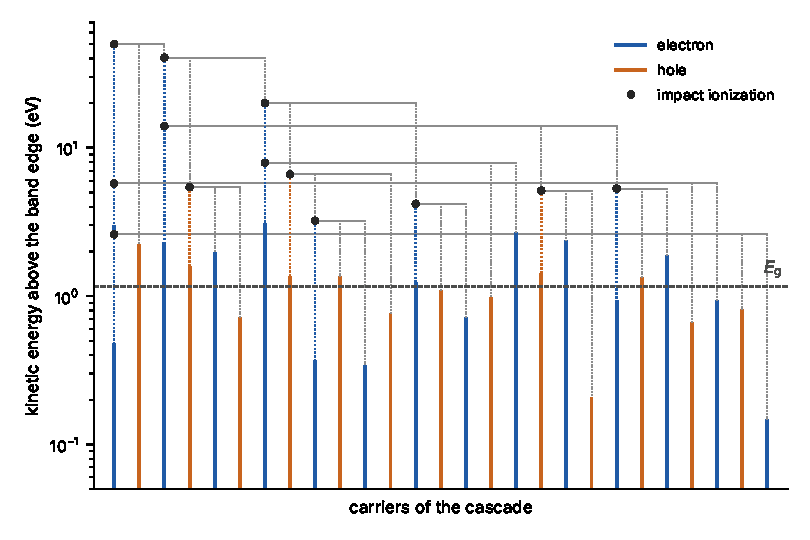
\includegraphics[width=0.95\linewidth]{figures/ch18/fig18_1.pdf}
  \caption{One sampled cascade started by an electron with \SI{50}{eV} of kinetic energy in silicon, in the energy-only random-$k$ model of \cref{sec:18.1-reductions}: free-particle densities of states, constant matrix elements, impact ionization above $\Eg = \SI{1.160}{eV}$ (silicon at \SI{123}{K}; threshold ratio $\theta_{\mathrm{ii}} = 1$), one optical phonon of \SI{63}{meV}, the rate ratio \cref{eq:18.1-randomk} with $A_{\mathrm{AB}} = \SI{5.703}{eV^3}$ (calibrated in \cref{sec:18.4}), and holes confined to the \SI{12}{eV} valence band. Each column is one carrier (blue electrons, orange holes), drawn from the kinetic energy at which it was created down to the band edge, on a logarithmic axis. Solid segments are runs of phonon emission; a dot marks an impact ionization, after which the carrier continues at the lower energy reached along the dotted segment, and the grey lines lead to the two carriers created in the ionization. This cascade has 13 ionizations, 27 carriers and 176 phonon emissions, every emission made by a carrier below \SI{6}{eV}, and leaves \SI{34.9}{eV} as heat. On average the model makes 12.99 new pairs, \SI{3.85}{eV} per pair at this energy, with a variance of 0.119 times the mean (generating function of \cref{sec:18.3}).}
  \label{fig:18-tree}
\end{figure}

\subsection{Impact ionization as a master-formula rate}\label{sec:18.1-ii}

A carrier in the Bloch state $n\vect{k}$, an electron in a conduction band or a hole in a valence band, interacts with every other charge of the crystal through the Coulomb potential. It is charged, so it couples to the total charge density $n_Z$ of electrons and nuclei, as a dark photon does (\cref{sec:8.4}). In a collision it gives a momentum $\vect{p}$ to the target and ends in a state $n'$, $\vect{k} - \vect{p}$; we write $\vect{p}$ for the momentum transfer of the carrier and keep $\vect{q}$ for the dark-matter momentum transfer that made the seed. Because the carrier is a Bloch wave and not a plane wave, the momenta $\vect{p} + \vect{G}$ for all reciprocal-lattice vectors $\vect{G}$ lead to the same final carrier state, and their amplitudes add. With $\vect{p}$ in the first zone, the amplitude to reach $n'$, $\vect{k} - \vect{p}$ and the target state $|f\rangle$ is
\begin{equation*}
  \frac{1}{\Vol}\sum_{\vect{G}}v_{\mathrm{C}}(|\vect{p}+\vect{G}|)\,\rho_{n'n}(\vect{k},-\vect{p}-\vect{G})\,\langle f|n_Z(\vect{p}+\vect{G})|i\rangle ,
\end{equation*}
with the overlap $\rho_{n'n}$ of \cref{eq:3.2-rho} in the place of the plane-wave overlap of a free projectile. This amplitude comes from the interaction \cref{eq:8.1-Hint} with one coupling row for each $\vect{G}$, the potential $\tilde V_{\vect{G}} = v_{\mathrm{C}}(|\vect{p}+\vect{G}|)\,\rho_{n'n}(\vect{k},-\vect{p}-\vect{G})$, and the target operators $n_Z(\vect{p}+\vect{G})$. The master formula \cref{eq:8.2-rate} then yields the rate directly, with two changes. The sum over final projectile states runs over the bands $n'$ and the first zone instead of over all momenta. And the final carrier state must be empty, which adds the factor $1 - f_{n',\vect{k}-\vect{p}}$. The response matrix that appears is $S_{\vect{G}\vect{G}'}(\vect{p},\omega)$ of the total charge, at the energy $\omega = \varepsilon_{n\vect{k}} - \varepsilon_{n',\vect{k}-\vect{p}}$ that the carrier loses.

The fluctuation--dissipation theorem turns this response into the screened interaction. With $R$ the retarded density response of \cref{sec:8.7}, at $\omega > 0$ the theorem reads $S = -2\,(1 + n_{\mathrm{B}}(\omega))\,(R - R^\dagger)/2\ii$ as a matrix in $\vect{G}$, the matrix form of the relation used in \cref{sec:8.7}, with $1/(1 - \ee^{-\beta\omega}) = 1 + n_{\mathrm{B}}(\omega)$. Sandwiched between Coulomb kernels, $R$ gives $v_{\mathrm{C}}Rv_{\mathrm{C}} = W^{\mathrm{scr}} - v_{\mathrm{C}}$ by \cref{eq:4.8-W}, and the bare $v_{\mathrm{C}}$ is real and diagonal and drops out of the anti-Hermitian part of $v_{\mathrm{C}}Rv_{\mathrm{C}}$. With the dielectric matrix of electrons and nuclei together in $W^{\mathrm{scr}}$:
\begin{keyresult}[Impact-ionization kernel]
\begin{equation}
  \varGamma_{\mathrm{ii}}(n\vect{k}) = -2\sum_{n'}\int_{\mathrm{BZ}}\frac{\dd^3p}{(2\pi)^3}\sum_{\vect{G}\vect{G}'}\rho_{\vect{G}}^*\,\Bigl[\frac{W^{\mathrm{scr}} - W^{\mathrm{scr}\dagger}}{2\ii}\Bigr]_{\vect{G}\vect{G}'}\!(\vect{p},\omega)\;\rho_{\vect{G}'}\;\bigl[1 - f_{n',\vect{k}-\vect{p}}\bigr]\bigl[1 + n_{\mathrm{B}}(\omega)\bigr] ,
  \label{eq:18.1-ii}
\end{equation}
with $\rho_{\vect{G}} = \rho_{n'n}(\vect{k},-\vect{p}-\vect{G})$ and $\omega = \varepsilon_{n\vect{k}} - \varepsilon_{n',\vect{k}-\vect{p}}$. Without the off-diagonal elements $\vect{G} \neq \vect{G}'$ the sum over $\vect{G}$ and the integral over the zone combine into one integral over all $\vect{p}$,
\begin{equation}
  \varGamma_{\mathrm{ii}}(n\vect{k}) \simeq \sum_{n'}\int\frac{\dd^3p}{(2\pi)^3}\,2v_{\mathrm{C}}(p)\,\bigl|\rho_{n'n}(\vect{k},-\vect{p})\bigr|^2\,L(\vect{p},\omega)\,\bigl[1 - f_{n',\vect{k}-\vect{p}}\bigr]\bigl[1 + n_{\mathrm{B}}(\omega)\bigr] ,
  \label{eq:18.1-iidiag}
\end{equation}
with $L$ the loss function \cref{eq:4.4-SL} of the total dielectric matrix at the unreduced momentum $\vect{p}$.
\end{keyresult}
\noindent For a hole the occupations are those of holes, $1 - f \to f$ in the valence bands. For a free-electron gas, $\rho = 1$ and \cref{eq:18.1-iidiag} is the out-scattering part of the lifetime \cref{eq:4.8-lifetime}: the step from \cref{sec:4.8} to here is the step from plane waves to Bloch waves and from the electron gas to a crystal with nuclei. The two terms of \cref{eq:18.1-ii} with $\vect{G} \neq \vect{G}'$ are local fields, and the master formula delivers them in their anti-Hermitian combination, which is real for any $W^{\mathrm{scr}}$, since $(W^{\mathrm{scr}} - W^{\mathrm{scr}\dagger})/2\ii$ is a Hermitian matrix and $\rho^\dagger A\rho$ is real for every Hermitian $A$. The element-wise imaginary part of $W^{\mathrm{scr}}_{\vect{G}\vect{G}'}$ agrees with the anti-Hermitian combination only when $W^{\mathrm{scr}}_{\vect{G}\vect{G}'} = W^{\mathrm{scr}}_{\vect{G}'\vect{G}}$, which holds in silicon and germanium with the origin at an inversion center but not in GaAs. The same symmetry condition separated the retarded and advanced pair weights of \cref{sec:8.7}.

The kernel is the rate at which the carrier scatters out of $n\vect{k}$. The quasiparticle width of the carrier differs from this out-scattering rate in two ways. By the cutting rule of \cref{sec:4.8}, $-2\Imag\Sigma^{\mathrm{R}} = \varGamma_{\mathrm{out}} + \varGamma_{\mathrm{in}}$. The in-scattering term carries the product $f\,n_{\mathrm{B}}$ of an occupied final state and a thermal excitation of energy $\omega \ge \Eg$, and so vanishes for a hot carrier at $T \ll \Eg$. The width also carries the quasiparticle residue, $\varGamma_{\mathrm{qp}} = -2z_{\mathrm{qp}}\Imag\Sigma^{\mathrm{R}}$ by \cref{eq:4.7-qp}, with $z_{\mathrm{qp}} \approx 0.8$ for the hot carriers of semiconductors~\cite[Sect.~II]{kotani2010impact}. \Cref{eq:18.1-ii} is first order in $W^{\mathrm{scr}}$ and sets $z_{\mathrm{qp}} = 1$. Since the factor $z_{\mathrm{qp}}$ lowers every impact-ionization rate by a nearly uniform 20 percent, a calibrated model absorbs it. The exchange of the carrier with the electron it excites is a vertex correction, absent from \cref{eq:18.1-ii} as it was from \cref{eq:4.8-lifetime}; it enters only beyond first order in $W^{\mathrm{scr}}$, and \cref{sec:18.5} lists it among the open problems.

The plasmon is inside the kernel. In silicon $\varepsilon_2$ is still 0.224 at the plasmon energy, where $\varepsilon_1$ vanishes (\cref{we:4-siplasmon}), so the plasmon peak carries the weight of electron--hole pairs. A carrier that ``emits a plasmon'' and the plasmon that ``decays into a pair'' are one term of \cref{eq:18.1-ii}, and a cascade built on \cref{eq:18.1-ii} must not add a separate plasmon channel. The plasmon becomes a particle of the cascade only where its pole is undamped and carries no pair weight, as in aluminum below the critical momentum $q_{\mathrm{c}}$ of \cref{sec:4.5}; it then needs a decay kernel of its own.

The loss function vanishes for $\omega < \Eg$ at $T \ll \Eg$, so a carrier must give up at least the gap. Energy conservation alone would let it ionize as soon as its kinetic energy $x$ above the band edge exceeds $\Eg$, but the three final carriers must also carry its crystal momentum. Take parabolic bands with an electron mass $m^*_{\mathrm{e}}$ and a hole mass $m^*_{\mathrm{h}}$. At the threshold energy, which is the lowest energy at which an electron can make a pair, the three products of the ionization move with a common velocity $\vect{u}$, so that no energy is spent on motion in their center-of-mass frame. Momentum conservation gives $m^*_{\mathrm{e}}\vect{v}_0 = (2m^*_{\mathrm{e}} + m^*_{\mathrm{h}})\vect{u}$ for an initial velocity $\vect{v}_0$, energy conservation $\tfrac12m^*_{\mathrm{e}}v_0^2 = \Eg + \tfrac12(2m^*_{\mathrm{e}} + m^*_{\mathrm{h}})u^2$, and eliminating $\vect{u}$ yields
\begin{equation}
  x_{\mathrm{th}} = \theta_{\mathrm{ii}}\Eg , \qquad \theta_{\mathrm{ii}} = \frac{2m^*_{\mathrm{e}} + m^*_{\mathrm{h}}}{m^*_{\mathrm{e}} + m^*_{\mathrm{h}}} ,
  \label{eq:18.1-theta}
\end{equation}
with $\theta_{\mathrm{ii}}$ the impact-ionization threshold ratio. Equal masses give $\theta_{\mathrm{ii}} = 3/2$; for a hole the two masses exchange places. In a real band structure the threshold is soft rather than sharp, because a crystal conserves momentum only up to $\vect{G}$ and the bands are not parabolic. Just above threshold few final states satisfy both conservation laws, and the computed rate scatters by large factors from one $\vect{k}$ to the next~\cite[Fig.~2]{kotani2010impact}.

\subsection{The phonon-emission kernel}\label{sec:18.1-ph}

The carrier also couples to the displacements of the nuclei, through the vertex $g_{mn\nu}(\vect{k},\vect{Q})$ of \cref{eq:6.2-g}. Take the phonon coordinate of branch $\nu$ at $\vect{Q}$ as the target operator and $g$ as the potential. The response of a harmonic phonon coordinate is $2\pi[(n_{\vect{Q}\nu} + 1)\delta(\omega - \omega_{\vect{Q}\nu}) + n_{\vect{Q}\nu}\delta(\omega + \omega_{\vect{Q}\nu})]$, and the master formula with the Pauli factor of the final carrier gives the out-scattering part of \cref{eq:6.3-ImFM}, the phonon kernel $\varGamma_{\mathrm{ph}}(n\vect{k})$ of \cref{eq:E.13-gph}. At detector temperatures only the emission term survives. The vertex is screened statically, as density-functional perturbation theory computes it, and the corrections to static screening are of higher order in $\omega_{\vect{Q}\nu}/\Eg$ (\cref{sec:6.2}).

In a polar crystal the two kernels overlap. The total dielectric matrix in $W^{\mathrm{scr}}$ contains the ionic response, and at $\omega$ near the longitudinal optical frequency $\omega_L$ its loss function has the Fr\"ohlich line: \cref{eq:18.1-ii} already contains the emission of a longitudinal optical phonon through the macroscopic field. The long-range vertex $g^L = \ii C_{\mathrm{F}}\rho_{mn}/Q$ of \cref{eq:6.2-frohlich} is the same Coulomb line, seen from the phonon side. The phonon kernel of a polar crystal must therefore use the short-range vertex alone $g^S = g - g^L$, the split that \cref{sec:6.2} introduced for Wannier interpolation. The subtraction removes exactly the Fr\"ohlich term of \cref{eq:18.1-ii} only if the calculations of the two kernels share the Born charges, $\varepsilon_\infty$ and $\omega_L$, the multipoles, the long-range cutoff, and the model of the ionic response itself. The Born charges, $\varepsilon_\infty$ and $\omega_L$ come from one calculation. If $g^L$ carries quadrupoles as well as dipoles, so must the ionic part of the dielectric matrix; otherwise only the dipole $g^L$ is subtracted. When $g^L$ is cut off over $\vect{G}$ by a Gaussian, the ionic head of $W^{\mathrm{scr}}$ at $\vect{p} = \vect{Q} + \vect{G}$ carries the same cutoff, or the Gaussian tail is counted twice. And the ionic part of $W^{\mathrm{scr}}$ must be restricted to the same model as $g^L$, which keeps only the macroscopic multipole head, with the same cutoff: a full ionic dielectric matrix over all $\vect{G}$, as density-functional perturbation theory gives it, also contains the short-range coupling, which $g^S$ would then count a second time. In silicon, with $Z^* = 0$, there is no Fr\"ohlich line, and the dipole term vanishes; the condition on the model of the ionic response still applies to the short-range ionic response if $W^{\mathrm{scr}}$ includes it.

The first phonon emission depends on the sector of the seed. A pair of the zero-phonon sector $\mathcal{P}_0$ leaves the dark-matter interaction dressed, with the weight $z_{\mathrm{qp}}(m)$ of \cref{sec:8.6}, and its first emission is the first step of the cascade, made by $\varGamma_{\mathrm{ph}}$. A pair of the sector $\mathcal{P}_+$ arrives with its phonon already emitted, and that phonon's energy goes to heat once; the cascade does not emit it again (\cref{sec:8.7}).
\begin{keyresult}[Cascade kernels]
Every kernel of the hot-carrier cascade is a rate of the master formula \cref{eq:8.2-rate} with a projectile from inside the target. Impact ionization has one coupling row per reciprocal-lattice vector, the potential $v_{\mathrm{C}}(|\vect{p}+\vect{G}|)\,\rho_{n'n}(\vect{k},-\vect{p}-\vect{G})$ and the response of the total charge, \cref{eq:18.1-ii}; phonon emission has the potential $g^S_{mn\nu}(\vect{k},\vect{Q})$ and the one-phonon response. Both kernels carry the Pauli factor of the final carrier state. The kernels hold at first order in $W^{\mathrm{scr}}$ and $g$, with $z_{\mathrm{qp}} = 1$ and the carrier distinguishable from the electrons it excites.
\end{keyresult}
\noindent The kernels for capture on an impurity and for the decay of a core hole by Auger emission have the same structure, with the impurity potential or the Coulomb interaction between bound and free states as the vertex; \cref{sec:18.5} treats capture.

\subsection{The cascade as a branching process}\label{sec:18.1-branching}

A cascade particle is in a state $x$: its type (electron or hole; a plasmon, a core hole or a trapped carrier where these occur), its band and its crystal momentum. In a collision of channel $c$ it turns into particles in the states $x'_1, \dots, x'_m$ at the rate density $\mathscr{K}_c(x \to x'_1\dots x'_m)$, read off the kernels above. Impact ionization turns one carrier into three: the carrier itself, at lower energy, and the electron and hole it created. Phonon emission turns one carrier into one and passes $\omega_{\vect{Q}\nu}$ to the lattice. The total rate out of $x$ is $\varGamma_x = \sum_c\int\mathscr{K}_c$. Each collision leaves an additive deposit $\delta\vect{N}_c$, a vector with one entry per quantity we count: one more pair for an ionization, $\omega_{\vect{Q}\nu}$ more heat for an emission. A carrier whose kinetic energy is below $\theta_{\mathrm{ii}}\Eg$ can no longer ionize. It relaxes to its band edge, and its kinetic energy is its last deposit of heat; capture and exciton formation, which change the relaxation to the band edge, are the subject of \cref{sec:18.5}.

The cascade is a branching process if collisions are Markovian, carriers evolve independently, and every line terminates; each of these three hypotheses can fail. The first is the Markov property: a collision is short compared with the time between collisions, and no coherence survives from one collision to the next. The Markov property is the incoherent limit, valid when the total rate of a carrier is small compared with its energy above the band edge, and least reliable within a width of the impact-ionization threshold. The second is that the carriers of one cascade evolve independently, with no Pauli blocking and no Coulomb interaction among them. Pauli blocking needs final-state occupations near one, in the states the hot carriers scatter into, a few eV above the band edges. With the conduction masses of \cref{tab:3-materials}, six valleys give a density-of-states mass of $1.06\,m_e$, and parabolic bands hold $7.5\times10^{21}$ states per \si{cm^3} per eV at \SI{1}{eV} above the edge. The estimate assumes that the pairs of a deposit share a sphere of radius \SI{10}{nm}; a \SI{1}{keV} deposit then makes 267 pairs at a density of $6.4\times10^{19}$ per \si{cm^3}, which fills less than $10^{-2}$ of the states within an eV. Blocking is negligible. The Coulomb interaction among the carriers is not negligible at the same density: with the exciton radius $a_x = \SI{4.2}{nm}$ of silicon (\cref{sec:4.9}), the pair density times $a_x^3$ is 4.7 at \SI{1}{keV} and 0.47 at \SI{100}{eV}. As a result, the independence hypothesis is marginal for the deposits of tens of eV that light dark matter makes, and for keV deposits it is an assumption whose error has not been estimated. The third hypothesis is termination: every particle reaches a terminal state with probability one. It holds because every collision lowers the energy of the colliding carrier and its products by at least the smallest phonon energy or the gap, at temperatures where absorption of phonons is negligible.

Under these hypotheses the statistics of the whole cascade follow from one generating functional. Let $\vect{N}$ be the total deposit of the cascade started by a particle in state $x$, with entries such as the pair number $N_{\mathrm{eh}}$ and the heat $E_{\mathrm{heat}}$, and let $\vect{\lambda}$ be a vector of conjugate variables of the same length. The \emph{branching generating functional} $\mathfrak{G}_x(\vect{\lambda}) = \langle\ee^{\vect{\lambda}\cdot\vect{N}}\,|\,x\rangle$ obeys
\begin{keyresult}[Backward equation of the cascade]
\begin{equation}
  \varGamma_x\,\mathfrak{G}_x(\vect{\lambda}) = \sum_c\int\dd x'_1\cdots\dd x'_m\;\mathscr{K}_c(x \to x'_1\dots x'_m)\;\ee^{\vect{\lambda}\cdot\delta\vect{N}_c}\prod_{j=1}^m\mathfrak{G}_{x'_j}(\vect{\lambda}) ,
  \label{eq:18.1-backward}
\end{equation}
with $\mathfrak{G}_x = \ee^{\vect{\lambda}\cdot\vect{N}_{\mathrm{term}}(x)}$ on the terminal states, whose deposit $\vect{N}_{\mathrm{term}}(x)$ is fixed. The physical solution is the minimal one, obtained by iterating from the terminal states.
\end{keyresult}
\noindent \Cref{app:D.43} derives the backward equation by first-step analysis: condition on the first collision, and the products start independent copies of the same process. The backward equation is the type-and-deposit functional \cref{eq:C.11-functional} of a branching process, with the branching ratios $\int\mathscr{K}_c/\varGamma_x$ in place of the probabilities $p_c$, written in the exponential form that suits deposits that are not integers. Time does not appear in the backward equation. Only the ratios of rates enter, because the cascade at a given energy depends on the order of the collisions and not on their timing; the absolute rates matter for the Markov hypothesis and for the timing of the signal. The minimality condition rules out the spurious fixed points that \cref{app:C.11} met in the toy branching law $1 - p + ps^2$, and in the cascade the minimality condition holds automatically, because every channel lowers the energy. The moments obey linear equations, \cref{eq:C.11-mean,eq:C.11-second} with the same substitution. Every term on the right-hand side of these equations refers to products of lower energy than $x$, so the equations are solved in a single sweep upward in energy.

Each collision conserves energy, and energy conservation ties the entries of $\vect{N}$ together. Without capture, excitons and escaping photons, a deposit $\omega$ that starts with one pair ends, in every event, as
\begin{equation}
  \omega = N_{\mathrm{eh}}\Eg + E_{\mathrm{heat}} ,
  \label{eq:18.1-energy}
\end{equation}
since each pair holds $\Eg$ once its carriers are at the band edges and all other energy has gone to phonons. For a carrier injected alone, with kinetic energy $x$, \cref{eq:18.1-energy} holds with $\omega \to x$ and $N_{\mathrm{eh}}$ counting the new pairs. Since the energy balance holds on every path, the joint functional of pairs and heat is fixed by the functional of the pairs alone, $\mathfrak{G}(\lambda_N, \lambda_H) = \ee^{\lambda_H\omega}\,\mathfrak{G}(\lambda_N - \lambda_H\Eg, 0)$, and every statement about the fluctuations of $N_{\mathrm{eh}}$ is a statement about the fluctuations of the heat. \Cref{sec:18.2} builds $\varepsilon_{\mathrm{eh}}$ and $F_{\mathrm{eh}}$ on this identity.

\begin{workedexample}{The generating function of a two-step toy cascade}\label{we:18-toy}
Measure energies in units of $\Eg$, take the threshold ratio $\theta_{\mathrm{ii}} = 3/2$, and let the only phonon carry $1/2$, far more than a real phonon, so that the cascade has at most two steps. A carrier at $x = 2$ ionizes with probability $p_a$; the three resulting carriers then share $x - 1 = 1$, all are below threshold, and the cascade ends. Otherwise, with probability $1 - p_a$, the carrier emits a phonon and is then at $x = 3/2$. There it ionizes with probability $p_b$, the products sharing $1/2$, or emits a second phonon and stops at $x = 1$, below threshold. Let $s = \ee^{\lambda_N}$ count new pairs. All products of the ionization at $3/2$ are terminal, with $\mathfrak{G} = 1$, so \cref{eq:18.1-backward} read from the bottom up gives $\mathfrak{G}_{3/2}(s) = p_bs + 1 - p_b$, and then
\begin{equation*}
  \mathfrak{G}_2(s) = p_a\,s + (1 - p_a)\,\mathfrak{G}_{3/2}(s) = p_a\,s + (1 - p_a)(p_b\,s + 1 - p_b) .
\end{equation*}
The heat is $2 - N_{\mathrm{eh}}$ on every path: an ionization at 2 leaves heat 1, at $3/2$ heat $1/2 + 1/2$, and two emissions heat $1/2 + 1/2 + 1$. Multiplying each path by $\ee^{\lambda_H E_{\mathrm{heat}}}$ gives $\ee^{2\lambda_H}\mathfrak{G}_2(s\,\ee^{-\lambda_H})$, the energy identity of the text.

Now seed the cascade with one pair whose electron and hole both start at $x = 2$ and follow the same rules. The seed pair counts once, and the two carriers are independent, so
\begin{equation*}
  \mathfrak{G}_\Lambda(s) = s\,\mathfrak{G}_2(s)^2 .
\end{equation*}
With $p_a = 3/5$ and $p_b = 2/5$, one carrier makes $\mathfrak{G}_2'(1) = 19/25$ new pairs on average. Expanding $\mathfrak{G}_\Lambda$ in powers of $s$ yields the probabilities of 1, 2 and 3 pairs, $36/625$, $228/625$ and $361/625$. The mean is $63/25 = 2.52$ and the variance $228/625 = 0.365$, so the deposit $\omega = 1 + 2 + 2 = 5$ costs $5/2.52 = 1.98$ gap energies per pair and the variance is 0.145 of the mean.
\end{workedexample}

\subsection{Energy-only and random-$k$ reductions}\label{sec:18.1-reductions}

The backward equation \cref{eq:18.1-backward} runs over every band and crystal momentum of every carrier, more states than a calculation can tabulate. The first reduction removes the momentum. Suppose that momentum-randomizing collisions, the scattering by intervalley and acoustic phonons, are much faster than the collisions that change the energy, $\varGamma_k \gg \varGamma_E$ with $\varGamma_E = \varGamma_{\mathrm{ii}} + \varGamma_{\mathrm{ph}}$ restricted to optical emission. These phonons carry a few tens of meV against the eV of a hot carrier, so they turn its momentum around while barely changing its energy. Between two energy-changing collisions a carrier then spreads uniformly over its surface of constant energy, and after its first collision its future depends only on its type $t$ and kinetic energy $x$: $\mathfrak{G}_{n\vect{k}} \to \mathfrak{G}_t(x)$. The kernels become iso-energy averages,
\begin{equation}
  \bar{\mathscr{K}}_t(x \to \dots) = \frac{\sum_{n\vect{k}}\delta(x - \varepsilon_{n\vect{k}})\,\mathscr{K}(n\vect{k} \to \dots)}{\sum_{n\vect{k}}\delta(x - \varepsilon_{n\vect{k}})} ,
  \label{eq:18.1-isoenergy}
\end{equation}
with $\varepsilon_{n\vect{k}}$ measured from the band edge of type $t$, and \cref{eq:18.1-backward} becomes a recursion in one variable per type. The same reduction follows from a second hypothesis, which does not need fast randomization. The second hypothesis is that the products of each ionization are spread over their energy surfaces independently of the momentum of the parent, as they nearly are when the momentum transfer $\vect{p}$ in \cref{eq:18.1-ii} ranges over many reciprocal-lattice vectors.

Neither hypothesis is safe in silicon. Above 3 to \SI{5}{eV}, impact ionization is as fast as phonon emission, and in the model of \cref{fig:18-tree} the two are equally likely at \SI{5.9}{eV}; there $\varGamma_E$ is no longer small against $\varGamma_k$, at exactly the energies where the number of ionizations is decided. The second hypothesis has not been proved. We expect an error of roughly $\varGamma_E/\varGamma_k$ per generation. This is an estimate, not a bound. The energy-only reduction does fix which carriers keep a memory of momentum. The seed carriers and the first products they make form the first generation, which keeps the crystal momenta it was born with and, through these momenta, the dark-matter momentum transfer $\vect{q}$ that made the seed. Every later generation sees energies alone.

A full-band calculation shows how the reductions compare with a calculation that keeps band structure and momentum. It treats the cascade in silicon with the kernels of \cref{sec:18.1-ii,sec:18.1-ph} on empirical pseudopotential bands, deformation-potential phonons and no fitted constant (\cref{sec:18.3-fullband}). The exchange factor of \cref{eq:18.1-ii} is the ratio of the full Kane rate to its direct part. The full-band calculation puts the exchange factor at 0.66 to 0.84 for electrons and 0.51 to 0.68 for holes above \SI{3}{eV}, inside the range of 0.5 to 1 that Kotani and van Schilfgaarde give~\cite[Eq.~(5)]{kotani2010impact}. The pair energy is decided by the competition of impact ionization and phonon emission between about 2.5 and \SI{4.5}{eV}: tripling the ionization rate below \SI{4.5}{eV} lowers $\varepsilon_{\mathrm{eh}}$ from 4.15 to \SI{3.73}{eV}, while doubling the rate above \SI{5}{eV} leaves $\varepsilon_{\mathrm{eh}}$ unchanged, since almost every carrier there ionizes either way. Near threshold phonon emission decides the count: at \SI{4}{eV} fewer than 1 percent of the events have two or more pairs, while without phonon emission nearly all would. And the momentum memory is negligible within the model: the full-band cascade and the same cascade with every carrier redrawn on its energy surface after each collision give nearly the same distributions. That comparison is internal to the deformation-potential model, in which every optical or intervalley emission redraws the crystal momentum anyway; the comparison tests only the memory of the first collision.

The second reduction, the random-$k$ approximation, replaces the matrix elements by constants and drops momentum conservation. Take the golden-rule form of impact ionization, a sum over the two final electrons and the hole with a squared screened matrix element, as written by Kane and quoted by Kotani and van Schilfgaarde~\cite[Eq.~(5)]{kotani2010impact}. With a constant matrix element and with every final momentum allowed, the sum is the three-body density of final states. Let $\rho_t(x)$ be the density of states of a carrier of type $t$ at kinetic energy $x$ and $\bar t$ the other type. A carrier of type $t$ at $x$ ionizes at a rate proportional to
\begin{equation}
  \mathfrak{P}_t(y) = \int_0^\infty\!\!\dd x_1\,\dd x_2\,\dd x_3\;\rho_t(x_1)\,\rho_t(x_2)\,\rho_{\bar t}(x_3)\;\delta(y - x_1 - x_2 - x_3) , \qquad y = x - \Eg ,
  \label{eq:18.1-phase}
\end{equation}
and its three products have the joint density $\rho_t(x_1)\rho_t(x_2)\rho_{\bar t}(x_3)/\mathfrak{P}_t(y)$ on the plane $x_1 + x_2 + x_3 = y$. The phonon rate is proportional to the density of states after one emission, $\rho_t(x - \omega_{\mathrm{AB}})$, for a single optical phonon of energy $\omega_{\mathrm{AB}}$. The ratio of the phonon rate to the ionization rate is
\begin{equation}
  \frac{\varGamma_{\mathrm{ph}}(x)}{\varGamma_{\mathrm{ii}}(x)} = A_{\mathrm{AB}}\,\frac{\rho_t(x - \omega_{\mathrm{AB}})}{\mathfrak{P}_t(x - \Eg)} ,
  \label{eq:18.1-randomk}
\end{equation}
with one constant $A_{\mathrm{AB}}$ that collects the two squared matrix elements. The threshold ratio is now $\theta_{\mathrm{ii}} = 1$, since momentum no longer constrains the products. For free-particle densities of states, $\rho_t(x) = x^{1/2}$, the integral \cref{eq:18.1-phase} is the Dirichlet integral $\int\prod_j x_j^{a-1}\,\delta(y - \sum_jx_j) = \Gamma(a)^3y^{3a-1}/\Gamma(3a)$ at $a = 3/2$. Since $\Gamma(3/2) = \sqrt\pi/2$ and $\Gamma(9/2) = 105\sqrt\pi/16$,
\begin{equation*}
  \mathfrak{P}(y) = \frac{\Gamma(3/2)^3}{\Gamma(9/2)}\,y^{7/2} = \frac{2\pi}{105}\,y^{7/2} ,
\end{equation*}
and \cref{eq:18.1-randomk} becomes the ratio \cref{eq:E.13-ab} of the model of Alig, Bloom and Struck, the Alig--Bloom model, as Ramanathan and Kurinsky implement it~\cite[Eq.~(8)]{ramanathan2020ionization}. With $\rho_t$ in $\mathrm{eV}^{1/2}$ and $\mathfrak{P}$ in $\mathrm{eV}^{7/2}$, $A_{\mathrm{AB}}$ carries $\mathrm{eV}^3$. We cut the hole density of states at the \SI{12}{eV} width of the silicon valence band~\cite[Sect.~III\,A]{ramanathan2020ionization}, so that a split with a hole above \SI{12}{eV} never occurs, and fix $A_{\mathrm{AB}}$ by the measured pair energy of silicon at \SI{123}{K}, where $\Eg = \SI{1.160}{eV}$; \cref{sec:18.4} derives the value, $A_{\mathrm{AB}} = \SI{5.703}{eV^3}$.

\Cref{fig:18-tree} is drawn with this model. The products of each ionization are sampled from the free-particle density, which is the scaled Dirichlet distribution with all three parameters $3/2$, and a hole drawn above \SI{12}{eV} is rejected. The rate ratio falls steeply with energy, and the cascade is decided by the competition between ionization and phonon emission at a few eV.

\subsection{Seeding the cascade}\label{sec:18.1-seed}

A dark-matter interaction leaves a final state of a class $\Lambda$ (\cref{sec:8.7}), typically an electron at $(E_{\mathrm{e}},\vect{k}_{\mathrm{e}})$ and a hole at $(E_{\mathrm{h}},\vect{k}_{\mathrm{h}})$, plus phonons or a core hole in other sectors. By the independence hypothesis the generating functional of the cascade that the final state starts is the product over the particles of the final state,
\begin{equation}
  \mathfrak{G}_\Lambda(\vect{\lambda}) = \ee^{\lambda_N}\,\mathfrak{G}_{\mathrm{e}}(E_{\mathrm{e}},\vect{k}_{\mathrm{e}};\vect{\lambda})\,\mathfrak{G}_{\mathrm{h}}(E_{\mathrm{h}},\vect{k}_{\mathrm{h}};\vect{\lambda}) ,
  \label{eq:18.1-seed}
\end{equation}
for a pair, with the seed pair counted by $\ee^{\lambda_N}$, as in \cref{we:18-toy}. \Cref{sec:18.3} builds $P_{\mathrm{casc}}(N_{\mathrm{eh}}|\Lambda)$ from \cref{eq:18.1-seed}.

Three properties of \cref{eq:18.1-seed} make the operator structure of the final state matter. First, at a fixed deposit $\omega$ the product depends on how $\omega - \Eg$ is split between the electron and the hole, and in the first generation on their crystal momenta. Second, $\mathfrak{G}_t$ is not linear in the carrier energy, so a cascade started from the average split is not the average of the cascades started from the actual splits. In the model of \cref{fig:18-tree}, a \SI{10}{eV} deposit whose \SI{8.84}{eV} above the gap is split equally yields 2.985 pairs on average and two pairs in \SI{4.5}{\percent} of events. A uniform distribution of splits, whose mean is the equal split, yields 2.691 pairs, and two pairs in \SI{36}{\percent} of events. Giving everything to the electron yields 3.003, with two pairs in \SI{14}{\percent}. At a few pairs the distribution of the split, not only its mean, sets the count. Third, the distribution of the split depends on the operator that made the pair and on $\vect{q}$: at \SI{10}{eV} in silicon the hole carries about \SI{0.9}{eV} more for a dark-matter kick at $q_0$ than for an absorbed photon (\cref{we:8-pairs}). The cascade has to be seeded class by class from the resolved response $S_{ab}(\vect{q},\omega;\Lambda)$, with the coupling tensor contracted inside the sum over classes, as the hand-off \cref{eq:8.7-handoff} requires. A seed distribution fitted to photon data at the same $\omega$ replaces the splits that the dark-matter operator makes at its momentum transfer by the splits that photon absorption makes.

The kernels are computed from first principles with the methods of \cref{app:E.13}: impact ionization from the $GW$ screened interaction on quasiparticle bands, with local fields, and phonon emission from vertices of density-functional perturbation theory interpolated with Wannier functions.
